% THIS IS SIGPROC-SP.TEX - VERSION 3.1
% WORKS WITH V3.2SP OF ACM_PROC_ARTICLE-SP.CLS
% APRIL 2009
%
% It is an example file showing how to use the 'acm_proc_article-sp.cls' V3.2SP
% LaTeX2e document class file for Conference Proceedings submissions.
% ----------------------------------------------------------------------------------------------------------------
% This .tex file (and associated .cls V3.2SP) *DOES NOT* produce:
%       1) The Permission Statement
%       2) The Conference (location) Info information
%       3) The Copyright Line with ACM data
%       4) Page numbering
% ---------------------------------------------------------------------------------------------------------------
% It is an example which *does* use the .bib file (from which the .bbl file
% is produced).
% REMEMBER HOWEVER: After having produced the .bbl file,
% and prior to final submission,
% you need to 'insert'  your .bbl file into your source .tex file so as to provide
% ONE 'self-contained' source file.
%
% Questions regarding SIGS should be sent to
% Adrienne Griscti ---> griscti@acm.org
%
% Questions/suggestions regarding the guidelines, .tex and .cls files, etc. to
% Gerald Murray ---> murray@hq.acm.org
%
% For tracking purposes - this is V3.1SP - APRIL 2009

\documentclass{acm_proc_article-sp}
\usepackage{amsmath, amsthm, amssymb, fancyhdr, enumerate}

\begin{document}

\title{Spike Sorting using Machine Learning}
\subtitle{Using unsupervised algorithms to automatically classify cells}
%
% You need the command \numberofauthors to handle the 'placement
% and alignment' of the authors beneath the title.
%
% For aesthetic reasons, we recommend 'three authors at a time'
% i.e. three 'name/affiliation blocks' be placed beneath the title.
%
% NOTE: You are NOT restricted in how many 'rows' of
% "name/affiliations" may appear. We just ask that you restrict
% the number of 'columns' to three.
%
% Because of the available 'opening page real-estate'
% we ask you to refrain from putting more than six authors
% (two rows with three columns) beneath the article title.
% More than six makes the first-page appear very cluttered indeed.
%
% Use the \alignauthor commands to handle the names
% and affiliations for an 'aesthetic maximum' of six authors.
% Add names, affiliations, addresses for
% the seventh etc. author(s) as the argument for the
% \additionalauthors command.
% These 'additional authors' will be output/set for you
% without further effort on your part as the last section in
% the body of your article BEFORE References or any Appendices.

\numberofauthors{3} %  in this sample file, there are a *total*
% of EIGHT authors. SIX appear on the 'first-page' (for formatting
% reasons) and the remaining two appear in the \additionalauthors section.
%
\author{
% You can go ahead and credit any number of authors here,
% e.g. one 'row of three' or two rows (consisting of one row of three
% and a second row of one, two or three).
%
% The command \alignauthor (no curly braces needed) should
% precede each author name, affiliation/snail-mail address and
% e-mail address. Additionally, tag each line of
% affiliation/address with \affaddr, and tag the
% e-mail address with \email.
%
% 1st. author
\alignauthor
David Brody\\
       \email{dbrody@stanford.edu}
% 2nd. author
\alignauthor Daniel Sommermann\\
       \email{dcsommer@stanford.edu}
% 3rd. author
\alignauthor
Michael Gummelt\\
       \email{mgummelt@stanford.edu}
}
\date{16 December 2011}
% Just remember to make sure that the TOTAL number of authors
% is the number that will appear on the first page PLUS the
% number that will appear in the \additionalauthors section.

\maketitle
\begin{abstract}
In this paper, we outline our approach to automatic spike sorting in the
context of electrical response from neurons. Using compression techniques
such as PCA and polynomial approximations, we were able to find a
tractable subspace in which to analyze our features. On our reduced
dimension samples, we then applied two algorithms wrapping k-means which
help find k: g-means clustering and using the Davies-Bouldin index. We
were able to get some 
very good clusters while other clusters were not as well separated,
indicating that there was a combination of a large degree of noise in our
features and high variability in terms of the response of each sensor when
a single cell spikes.

\end{abstract}

\section{Introduction}

Lab equipment gathers extracellular neurophysicological voltage samples at
a rate of 10 kHz. These readings are a mixture of the responses from the
many surrounding cells. The responses are then clustered into
similar shaped groups which represent different cells. Our
project aims to take this analysis step which is usually done
manually and automate it using machine learning. To gather the data for
our experiments, we recorded 100 seconds of data. The data is
extracellular recordings from 60 different channels. Each channel 
represents a data stream of voltage potentials at a specific microelectrode. A sample
recording looks like the following:

\begin{center}
  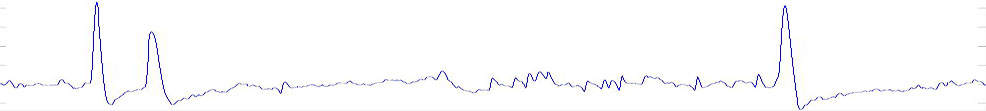
\includegraphics[width=0.8\linewidth]{../poster/images/voltagetrace_2_small.jpg}
\end{center}

The aim of the project is to cluster each spike into clusters
which each share a similar shape.  Example cluster centers
could look like the following:

\begin{center}
  \begin{tabular}{c c c}
    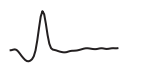
\includegraphics[width=0.17\linewidth]{../poster/images/WaveShape1.png} &
    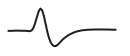
\includegraphics[width=0.17\linewidth]{../poster/images/WaveShape2.png} &
    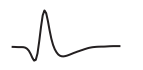
\includegraphics[width=0.17\linewidth]{../poster/images/WaveShape3.png}
  \end{tabular}
\end{center}

\section{Algorithmic Exploration}
\subsection{Model}
\noindent{\textbf{Model Parameters}}

N = \# of datapoints per channel

CH = \# of channels

S = \# of points to smooth raw data over

T = Threshold for spikes

L = \# points to take from left of spike location

R = \# points to take from right of spike location

\noindent{\textbf{Definitions}}
We begin with the raw waveform:
$$R = \{ {R \in \mathbb{R}^{N \times CH}; i = 1,...,CH} \}$$
Smoothing over S points we define a new waveform where $R^i_j$
is the jth datapoint in the ith channel: 
$$W^i_j = \frac{1}{s}\sum_{s=-S/2}^{S/2}R^{(i)}_{j+s}$$
We then define $W'$ as the zero mean normalized to the standard
deviation on each channel of $W$. The next step is to
separate out the possible spikes to cluster. We define the
spike locations of interest as:
$$P = \{ i; \frac{\partial}{\partial W} = 0 \cap 
  (W_1'(P_i) > T \cup ... \cup W_{CH}'(P_i) > T) \cap i \in
  1,...,N \} $$
Peaks are then cut to ensure that they are a minimum of
$\alpha = 15$ from each other. To form a single feature vector $X^{(i)}$ we take the
 surrounding points on each channel and concatentate them.
 $$X^{(i)}_j = W'^{floor(i/(L+R+1))+1}_{mod(j, L+R+1) + P(i)}
  ; i = 1,...,|P|, j = 1,...,(L+R+1)*CH$$
  $$X^{(i)} \in \mathbb{R}^{CH(L+R+1)}$$
$X$ is the feature vector we use to then cluster on.

\subsection{Process Overview}

For reference, the high level overview of our process pipeline is shown
below: 
\begin{center}
  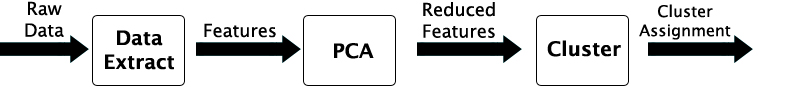
\includegraphics[width=0.8\linewidth]{../poster/images/pipeline.jpg}
\end{center}

We paramaterize our feature vectors from the raw data with the following representations:
$$X = M(R; S,T,L,R)$$
We then use different methods to reduce the dimensionality of
the feature vectors to improve performance and to emphasize
more discrimanent features.
  $$Red(X,N,M; X^{(i)} \in \mathbb{R}^N) = (Y^{(i)} \in
  \mathbb{R}^M,I^{(i)} \in \mathbb{R})$$
Clustering then takes the dimension reduced feature vectors
and assigns them to clusters which represent possible cells.

\subsection{Dimensionality reduction and compression}
\subsubsection{PCA}
At this point, we have our features and are ready to run unsupervised
learning algorithms on the data set. However, as we began experimenting
with our data set, we realized that the time needed to learn on our data
set was simply too great. We needed a way to reduce the dimensionality of
our features. Since a feature vector consists of 30 measurements for 60
channels each, we have features in $\mathbb{R}^{1800}$.

The first approach we took was to apply PCA and take the top 300 principal
components and project our features into that space, $\mathbb{R}^{300}$.

Performing this optimization allowed us to run k-means clustering in 13\%
of the time without compression. We experimented with projecting into
different dimension subspaces and found 300 to be a good dimension that
saves enough on running time without sacrificing too much in terms of
underfitting.

\begin{figure}
\centering
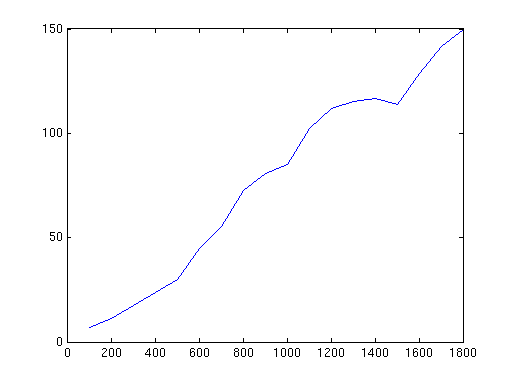
\includegraphics[width=3in,height=2in]{../poster/images/dim_vs_runningtime.png} 
\caption{This plot of the time clustering took (using g-means) vs the
  dimension we reduced to using PCA shows the roughly linear relationship 
between dimensionality of our feature vector and running
time.}
\end{figure}

Here we can clearly see the relationship between the dimensionality of our
featuer vectors and the time it takes to run our clustering code. As we
iterated on our project, reducing the running time of our algorithm was
critical to being able to try many different ideas quickly.

\subsubsection{Fitting Polynomials}

Another approach to reducing the dimensionality was to take
into account the dependencies of the features within each
channel. Since these values are continuous we can fit a
polynomial model to them with fewer parameters. Here we let $n$
be the number of coefficients we want to fit per channel. Since
we have 60 channels the end result is $\mathbb{R}^{60(n+1)}$
since the intercept parameter must be included per channel as well.

Our results with polynomial fitting were not as strong as
PCA. While they do a good job of making sure each channel is
fit well, the condensed features must encode all the
information unlike PCA where the principle components hold the
information. As a result, it takes many more features to get
the same amount of information back.

\begin{figure}
\centering
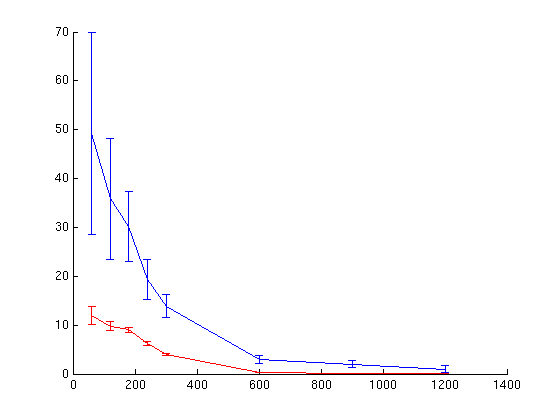
\includegraphics[width=3in,height=2in]{../poster/images/error_poly_pca.png}
\caption{This plot compares the error of the compression techniques we
  used. In blue is polynomial fitting and in red is PCA. The plot is of
  the percentage error vs dimension we reduce to.}
\end{figure}

While polynomial fitting does take temporal information into
account per channel in the condensation, it fails to encode the
meaningful information as well.

\subsection{Clustering Algorithms}
As the engine for both of the clustering algorithms, we used kmeans
clustering. However, the real work at this stage is to determine which k
should be used in kmeans. We tried two approaches to solving this
problem. 

\subsubsection{G-Means algorithm}
One way to choose k in the k-means algorithm is to use an algorithm
developed in 2003 by Greg Hamerly and Charles Elka, presented in the NIPS
2003 conference \cite{gmeans}. In this method, a small value for k is
chosen and kmeans is run. Then, for each cluster produced, we use a
heuristic function to decide whether to split that cluster. The heuristic
used is the Anderson-Darling statistic. If that statistic is greater than
some threshold critical value, then we decide that the cluster should be
split. The Anderson-Darling statistic is computed as follows:
$$
A^2(Z) = -n - \frac{1}{n}\sum_{i=1}^n (2i -
1)[\log(z_i)+\log(1-z_{n+1-i})]
$$$$
A^2_*(Z) = A^2(Z)(1 + 4/n - 25/n^2)
$$
If the $A^2_*(Z)$ is greater than the threshold, we split. For this
project we experimented with many thresholds and found that with $t=12$ we
got good separation between clusters.

\begin{figure}
\centering
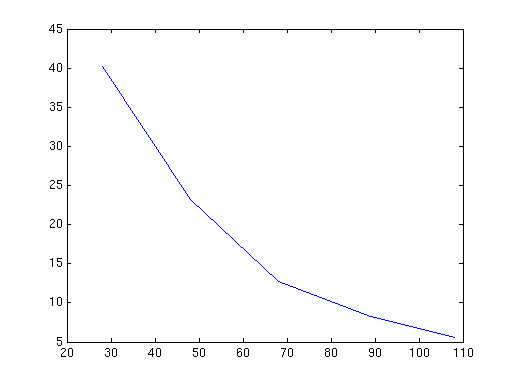
\includegraphics[width=1.3in,height=1in]{../poster/images/gmeans_k_vs_metric.png} 
\caption{The Anderson-Darling statistic is computed per cluster, so to
  show how it improves, we take the average value across all clusters and
  for each $k$ plot the mean here.}
\end{figure}


\subsubsection{Davies-Bouldin Index}
The DB Index is
another way to determine $k$ by favoring sets of clusters
with high intra-cluster similarity and low inter-cluster
similarity.  The formula is as follows:

$A^j$ = Center of cluster j

$T^j = \{ {X^{(i)} ; X^{(i)} \text{is in cluster} j} \}$

$S^i$ = the intra cluster similarity of cluster $i$

$M^{ij}$ = inter cluster similarity of clusters $i$, $j$

$S^i = (\frac{1}{|T^i|} \sum\limits_{j=1}^{|T^i|} (T^i_j -A^i)^q)^{\frac{1}{q}}$

$M^{ij} = (\sum\limits_{k=1}^{N} |a^i_k - a^j_k|^p)^{\frac{1}{p}}$

$DB = \frac{1}{N} \sum\limits_{i=1}^N \max_{j:i \neq j} R_{ij}$

\begin{figure}
\centering
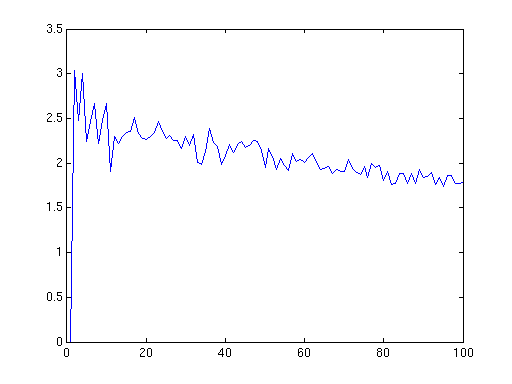
\includegraphics[width=1in,height=1in]{../poster/images/davies_k_vs_davies_index.png}
\caption{The graph above shows k vs the Davies-Bouldin Index}
\end{figure}

%\begin{figure*}
%\centering
%
\includegraphics[width=1in,height=1in]{sns.jpg}
%\caption{A sample black and white graphic (.eps format)
%that needs to span two columns of text.}
%\end{figure*}

\section{Conclusions}
PCA was very useful for compressing the data well.

Understanding meaning of data and how to format it correctly is important.

The number of clusters and the confidence of them is very dependent on the
heuristic used. 

Performing unsupervised learning with real world data is difficult.

Choosing right heuristic for clustering is important

\subsection{Future Work}
Using polynomial fitting then PCA to compress.

Use better clustering algorithm to take specific
            neurophysiological heuristics into account.


%\end{document}  % This is where a 'short' article might terminate

%
% The following two commands are all you need in the
% initial runs of your .tex file to
% produce the bibliography for the citations in your paper.
\bibliographystyle{abbrv}
\bibliography{sigproc}  % sigproc.bib is the name of the Bibliography in this case
% You must have a proper ".bib" file
%  and remember to run:
% latex bibtex latex latex
% to resolve all references
%
% ACM needs 'a single self-contained file'!
%

\end{document}
